\documentclass{beamer}
\usepackage{graphicx}
\usepackage{amsmath}
\usepackage{amssymb}
\usepackage{amscd} % Required for inserting images
\usetheme{metropolis}
\metroset{block=fill} 

\title{Modélisation d'Aptamères d'ADN IFT 3710}
\author{Dereck Piché, Jonas Gabirot, Guillermo Martinez}
\institute{Université de Montréal}
\date{Avril 2023}


\begin{document}

\frame{\titlepage}

\section{Contexte}

\begin{frame}{Contexte}
Les aptamères (du latin \emph{aptus} signifiant attaché) sont des séquences synthétiques d'ADN qui s'attachent à des molécules cibles soit pour les détecter, soit pour les neutraliser. Leur spécifité leur permet de s'attacher seulement à la cible voulue sans affecter leur environment.
\end{frame}


\begin{frame}{Contexte}
L'énergie libre est une propriété des molécules qui représentent la capacité à "activer" des réactions de façon spontanée. 

Un aptamère doit avoir une énergie libre correspondante à celle de la molécule cible pour s'y attacher. C'est une propriété nécessaire mais non suffisante.
\end{frame}


\begin{frame}{Objectif}
Cependant, les molécules d'ADN sont assez larges et le calcul de l'énergie libre devient très complexe lorsque la taille des molécules augmentent. Notre objectif est donc d'entraîner un modèle capable de prédire l'énergie d'une séquence d'ADN quelconque, afin d'accélérer la recherche d'aptamère.
\end{frame}


\section{Baseline: MLP}
\begin{frame}{MLP}

Comme baseline, nous avons choisi un réseau MLP standard. Les MLPs ne font aucune supposition sur la structure de la séquence, ce qui permet de comparer avec d'autres modèles qui se basent sur des hypothèses différentes. Ils sont aussi faciles à implémenter et entraîner. 
\begin{equation*}
    \begin{CD}
        @. Seq \in R^{120}
        @>Lin. (\times 20)>> 
        @>ReLU (\times 20)>> 
        @>Lin.>> 
        Energie \in R
    \end{CD}
\end{equation*}

\begin{block}{Hyperparamètres}
\begin{enumerate}
    \item Taux d'apprentissage: 0.0003
    \item Nombre de paramètres: 1 005 241
\end{enumerate}
\end{block}

\end{frame}


\begin{frame}{Résultats du MLP}
\begin{figure} \label{fig:mlp}
    \caption{Précision du MLP selon MSE} \center
    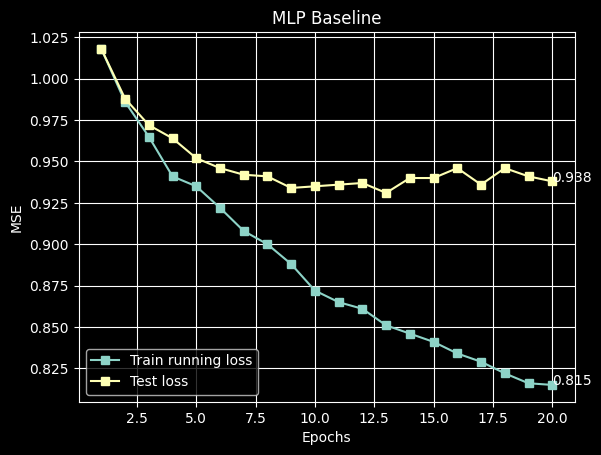
\includegraphics[width=0.7\textwidth]{images/mlp.png}
\end{figure}
\end{frame}


\section{Long Short Term Memory (LSTM)}

\begin{frame}{LSTM}
Le modèle LSTM (Long Short-Term Memory) est une variante des réseaux de neurones récurrents (RNN) qui permet de mieux gérer les problèmes liés à la mémoire à long terme. Il utilise des portes, qui sont des fonctions non linéaires, pour contrôler l'information qui entre ou sort de la mémoire.
\end{frame}


\begin{frame}{Portes}

Il y a trois types de portes : la porte d'oubli (forget gate) permet au modèle de décider ce qu'il faut oublier de la mémoire à long terme, la porte d'entrée (input gate) permet d'ajouter de nouvelles informations à la mémoire à long terme et la porte de sortie (output gate) permet de déterminer quelle information doit être renvoyée en sortie.
\begin{figure} \label{fig:architecture_lstm}
    \caption{Architecture LSTM} \center
    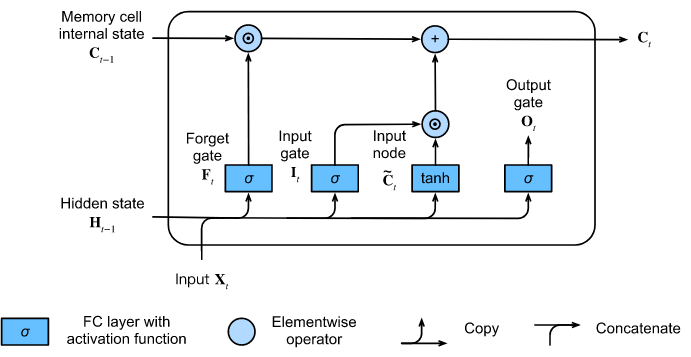
\includegraphics[width=0.6\textwidth]{images/lstm-schema.png}
\end{figure}

\end{frame}

\begin{frame}{Architecture du LSTM}

\begin{equation*}
    \begin{CD}
        @. Seq \in R^{120}
        @>LSTM1>> 
        @>LSTM2>> 
        @>Lin.>> 
        Energie \in R
    \end{CD}
\end{equation*}

\begin{block}{Hyperparamètres}
\begin{enumerate}
    \item Taux d'apprentissage: 0.0003
    \item Nombre de paramètres: 1 008 991 
    \item Dropout: 0.6
\end{enumerate}
\end{block}

\end{frame}

\begin{frame}{Résultats du LSTM}

\begin{figure} \label{fig:lstm}
    \caption{Précision du LSTM selon MSE} \center
    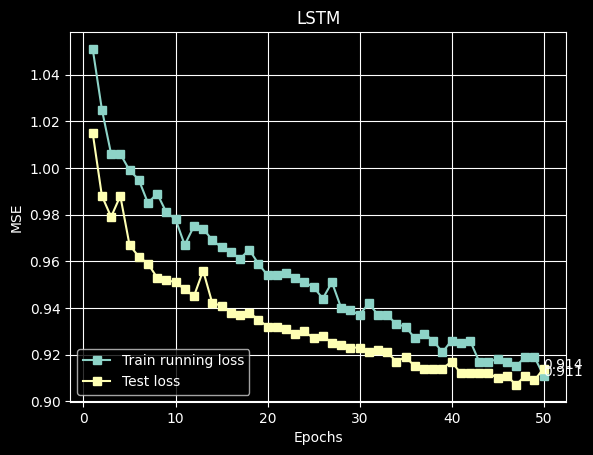
\includegraphics[width=0.7\textwidth]{images/lstm.png}
\end{figure}

\end{frame}
\section{Transformeurs}

\begin{frame}{Attention}
Un système d'attention retourne une somme des vecteurs \emph{Valeurs} selon 
une mesure de similarité entre les vecteurs \emph{Requêtes} et les vecteurs \emph{Clés}.
Cette mesure de similarité est appelée l'attention.
    \begin{block}{Système d'attention}
        $\sum_{j} a(q, k_j) v_j$
    \end{block}
Les transformeurs utilisent un système d'auto-attention, qui vise à produire
une séquence transformée dans laquelle chaque jeton est codé en effectuant une somme pondérée des
autres jetons présents dans sa séquence (l'incluant).
    \begin{block}{Jeton codé}
        $t_{i}^{'} = \sum_{j} a(W^{q}t_{i}, W^{k}t_j) W^{v}t_j$
    \end{block}
\end{frame}

\begin{frame}{Attention}
Dans les transformeurs, on utilise une attention spéciale :
\begin{block}{Attention au produit scalaire mis à l'échelle}
    \[ a(q, k) = softmax( \frac{q^Tk}{\sqrt{d}}) \]
\end{block}


{\bf Pourquoi le produit scalaire?}
On sait déjà que le produit scalaire peut être vu comme une mesure de la similarité entre
les deux vecteurs. Cela permet beaucoup de liberté au transformeur, qui obtient les vecteurs clés et les vecteurs requêtes en fonction des vecteurs jetons avant d'effectuer le produit scalaire. On le laisse donc créer sa propre mesure de distance, en quelque sorte.

\end{frame}

\begin{frame}{}
    
{\bf Pourquoi le softmax?}
Pour que les coéfficients somment à 1. (*expliquer l'intuition)

{\bf Pourquoi la division par la racine de la taille? }
Pour éviter des erreurs numériques. On épargne les détails.

\end{frame}

\begin{frame}{Couche de codage}
    Une tête d'attention retourne donc une séquence de la même taille que son entrée (sauf exceptions).
    Une couche de codage contient plusieurs têtes d'attention! Les sorties de ces 
    têtes d'attention sont concaténées dans {\it un gros vecteur} et on applique une transformation 
    linéaire (avec activation ReLU pour obtenir de l'expressivité non linéaire) à ce vecteur pour obtenir une sortie 
    de dimension arbitraire.
\end{frame}

\begin{frame}{Architecture du transformeur}
\begin{figure} \label{fig:transformer}
    \caption{Transformer de traduction dans AIAYN} \center
    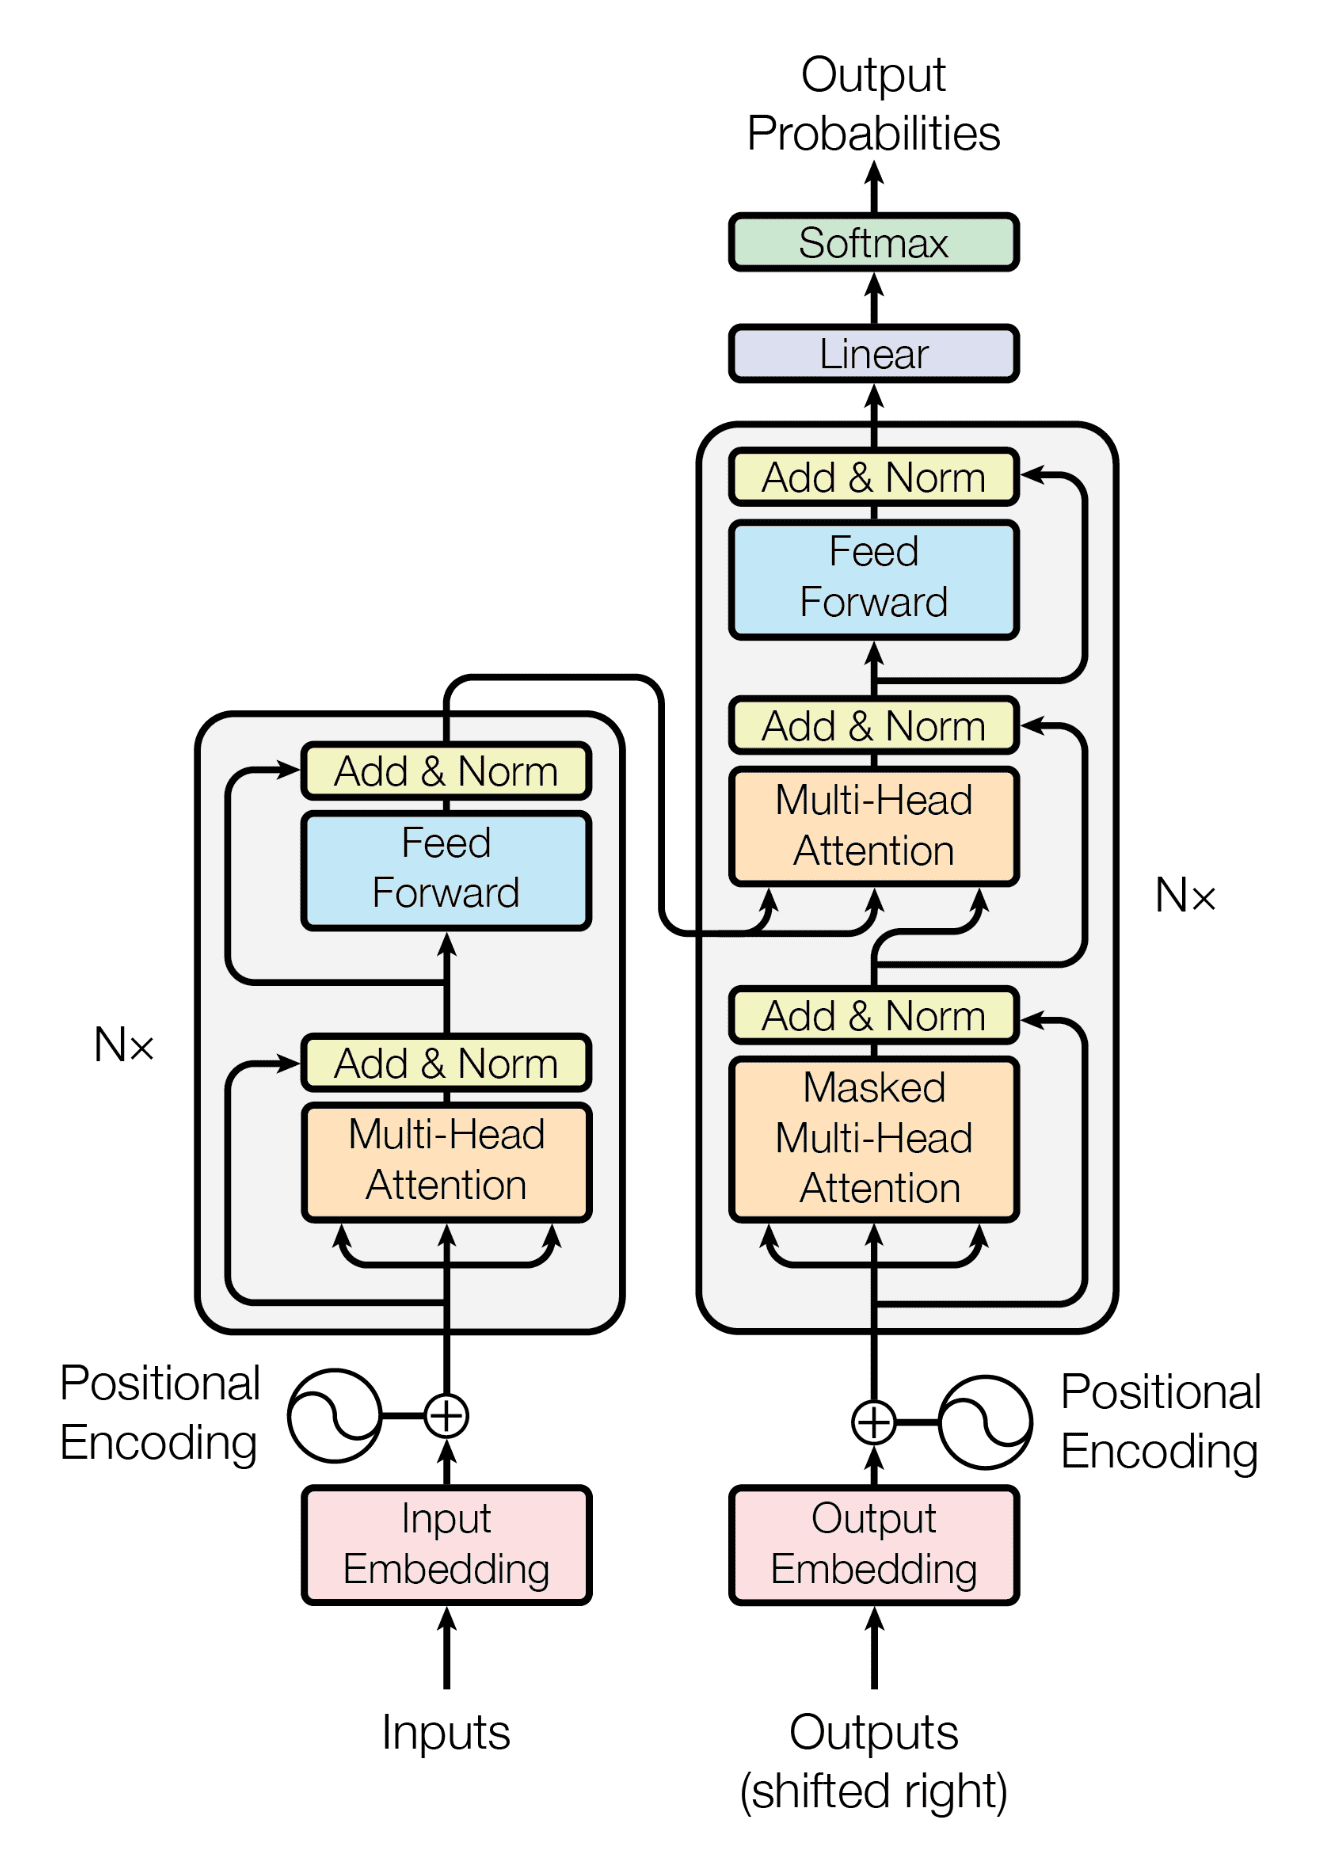
\includegraphics[width=0.5\textwidth]{images/2023-04-04-14-37-09.png}
\end{figure}
\end{frame}

\begin{frame}{Architecture du transformeur}
\begin{equation*}
    \begin{CD}
        @. Seq \in R^{30}
        @>Emb.>> 
        @>Cod. (\times 3)>> 
        @>Lin.>> Energie \in R
    \end{CD}
\end{equation*}

\begin{block}{Hyperparamètres}
\begin{enumerate}
    \item Taux d'apprentissage: $10^{-4}$
    \item Dimension d'embedding: 16
    \item Nombre de têtes: 8
    \item Nombre de paramètres: 1 786 753 
    \item Codage positionnel: sincos (AIAYN)
\end{enumerate}
\end{block}
\end{frame}


\begin{frame}{Résultats du transformeur}
\begin{figure} \label{fig:transformer_accuracy}
    \caption{Précision du transformeur selon MSE} \center
    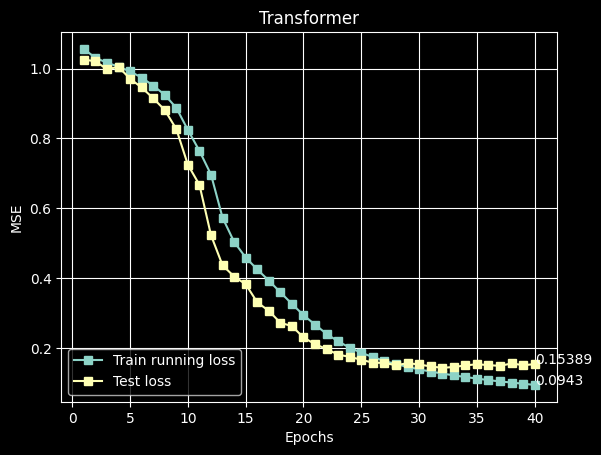
\includegraphics[width=0.7\textwidth]{images/2023-04-02-13-48-49.png}
\end{figure}
\end{frame}
\begin{frame}{Comparaison des résultats}
\begin{figure}
    \caption{MSE des 3 modèles} \center
    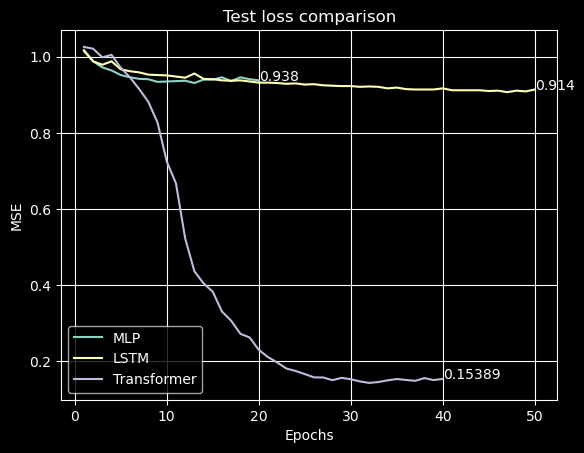
\includegraphics[width=0.7\textwidth]{images/comparaison.png}
\end{figure}
\end{frame}


\end{document}
